\chapter{Analýza a implementace serverové části}\label{ch:server}

\chaptersummary{
   \begin{ul}
      \item popis architektury serverové aplikace a metod zvolených pro realizaci,
      \item volba úložiště zdrojových kódů,
      \item rozbor komplexnějších funkcionalit a aspektů realizace.
   \end{ul}
}

Implementace serverové části na základě zadání a definované specifikace \g{IS} spočívá v anaýze aktuální monolitické architektury (z předchozí práce) a její přespis do architektury mikroslužeb s využitím zkušeností získaných a popsaných v kapitolách~\enquote{\nameref{ch:msa-intro}} a~\enquote{\nameref{ch:msa-data}}.

Ačkoliv původní implementace měla vyřešeno dost aspektů z hlediska funkcionality, přechod na novou architekturu způsobem využití exitujícíh zdrojových kódů by odhadem zabral víc času, než nová realizace s pouhou inspirací z původního systému.
Z tohoto důvodu bylo rozhodnuto napsat nový základ pro mikroslužby, který by víc vyhovoval aktuálním potřebám.
Pro novou relizaci bylo rovněž vybráno jiné \g{ORM}, které přineslo zjednodušení během vývoje za cenu změny implementace většiny funkcionalit spojených s relační databází.
Detailní popis změn a přínosů je uveden v následujících podkapitolách.

\newpage

\section{Architektura}\label{sec:server-arch}

Základním krokem pro návrh architektury serverové části se stal výběr typu dekompozice poskytnuté specifikace.


Při modelování poskytnuté domény do \g{MSA} je vhodné použít dekompozici úlohy na menší části s následujícím mapováním na služby.

Dekompozice se provedla na následující mikroslužby:



\begin{ul}
   \item \textbf{ms-users} – uživatelská data
   \item \textbf{ms-auth} – autentizační data, kontrola validity autorizačních údajů,
   \item \textbf{ms-projects} – služba pro správu projektovách dat.
   Ukládá v relační databázi metadata o projektech a deleguje úpravy obsahů na vnější Git úložiště
   \item \textbf{ms-interpreters} – správa registovaných interpretů
   \item \textbf{ms-communication} – zpracovávání komunikačních zpráv s uživateli
   \item \textbf{ms-monitoring} – služba pro centrální kontrolování stavů mikroslužeb
\end{ul}

A pomocné organizační služby:

\begin{dl}
   \item[Router-orch] – služba řízení dotazů na mikroslužby ve vnitřní komunikaci,
   \item[Gateway] – služba řízení dotazů na mikroslužby z vnějšího prostředí,
\end{dl}

\begin{figure}[htbp]
   \centering
   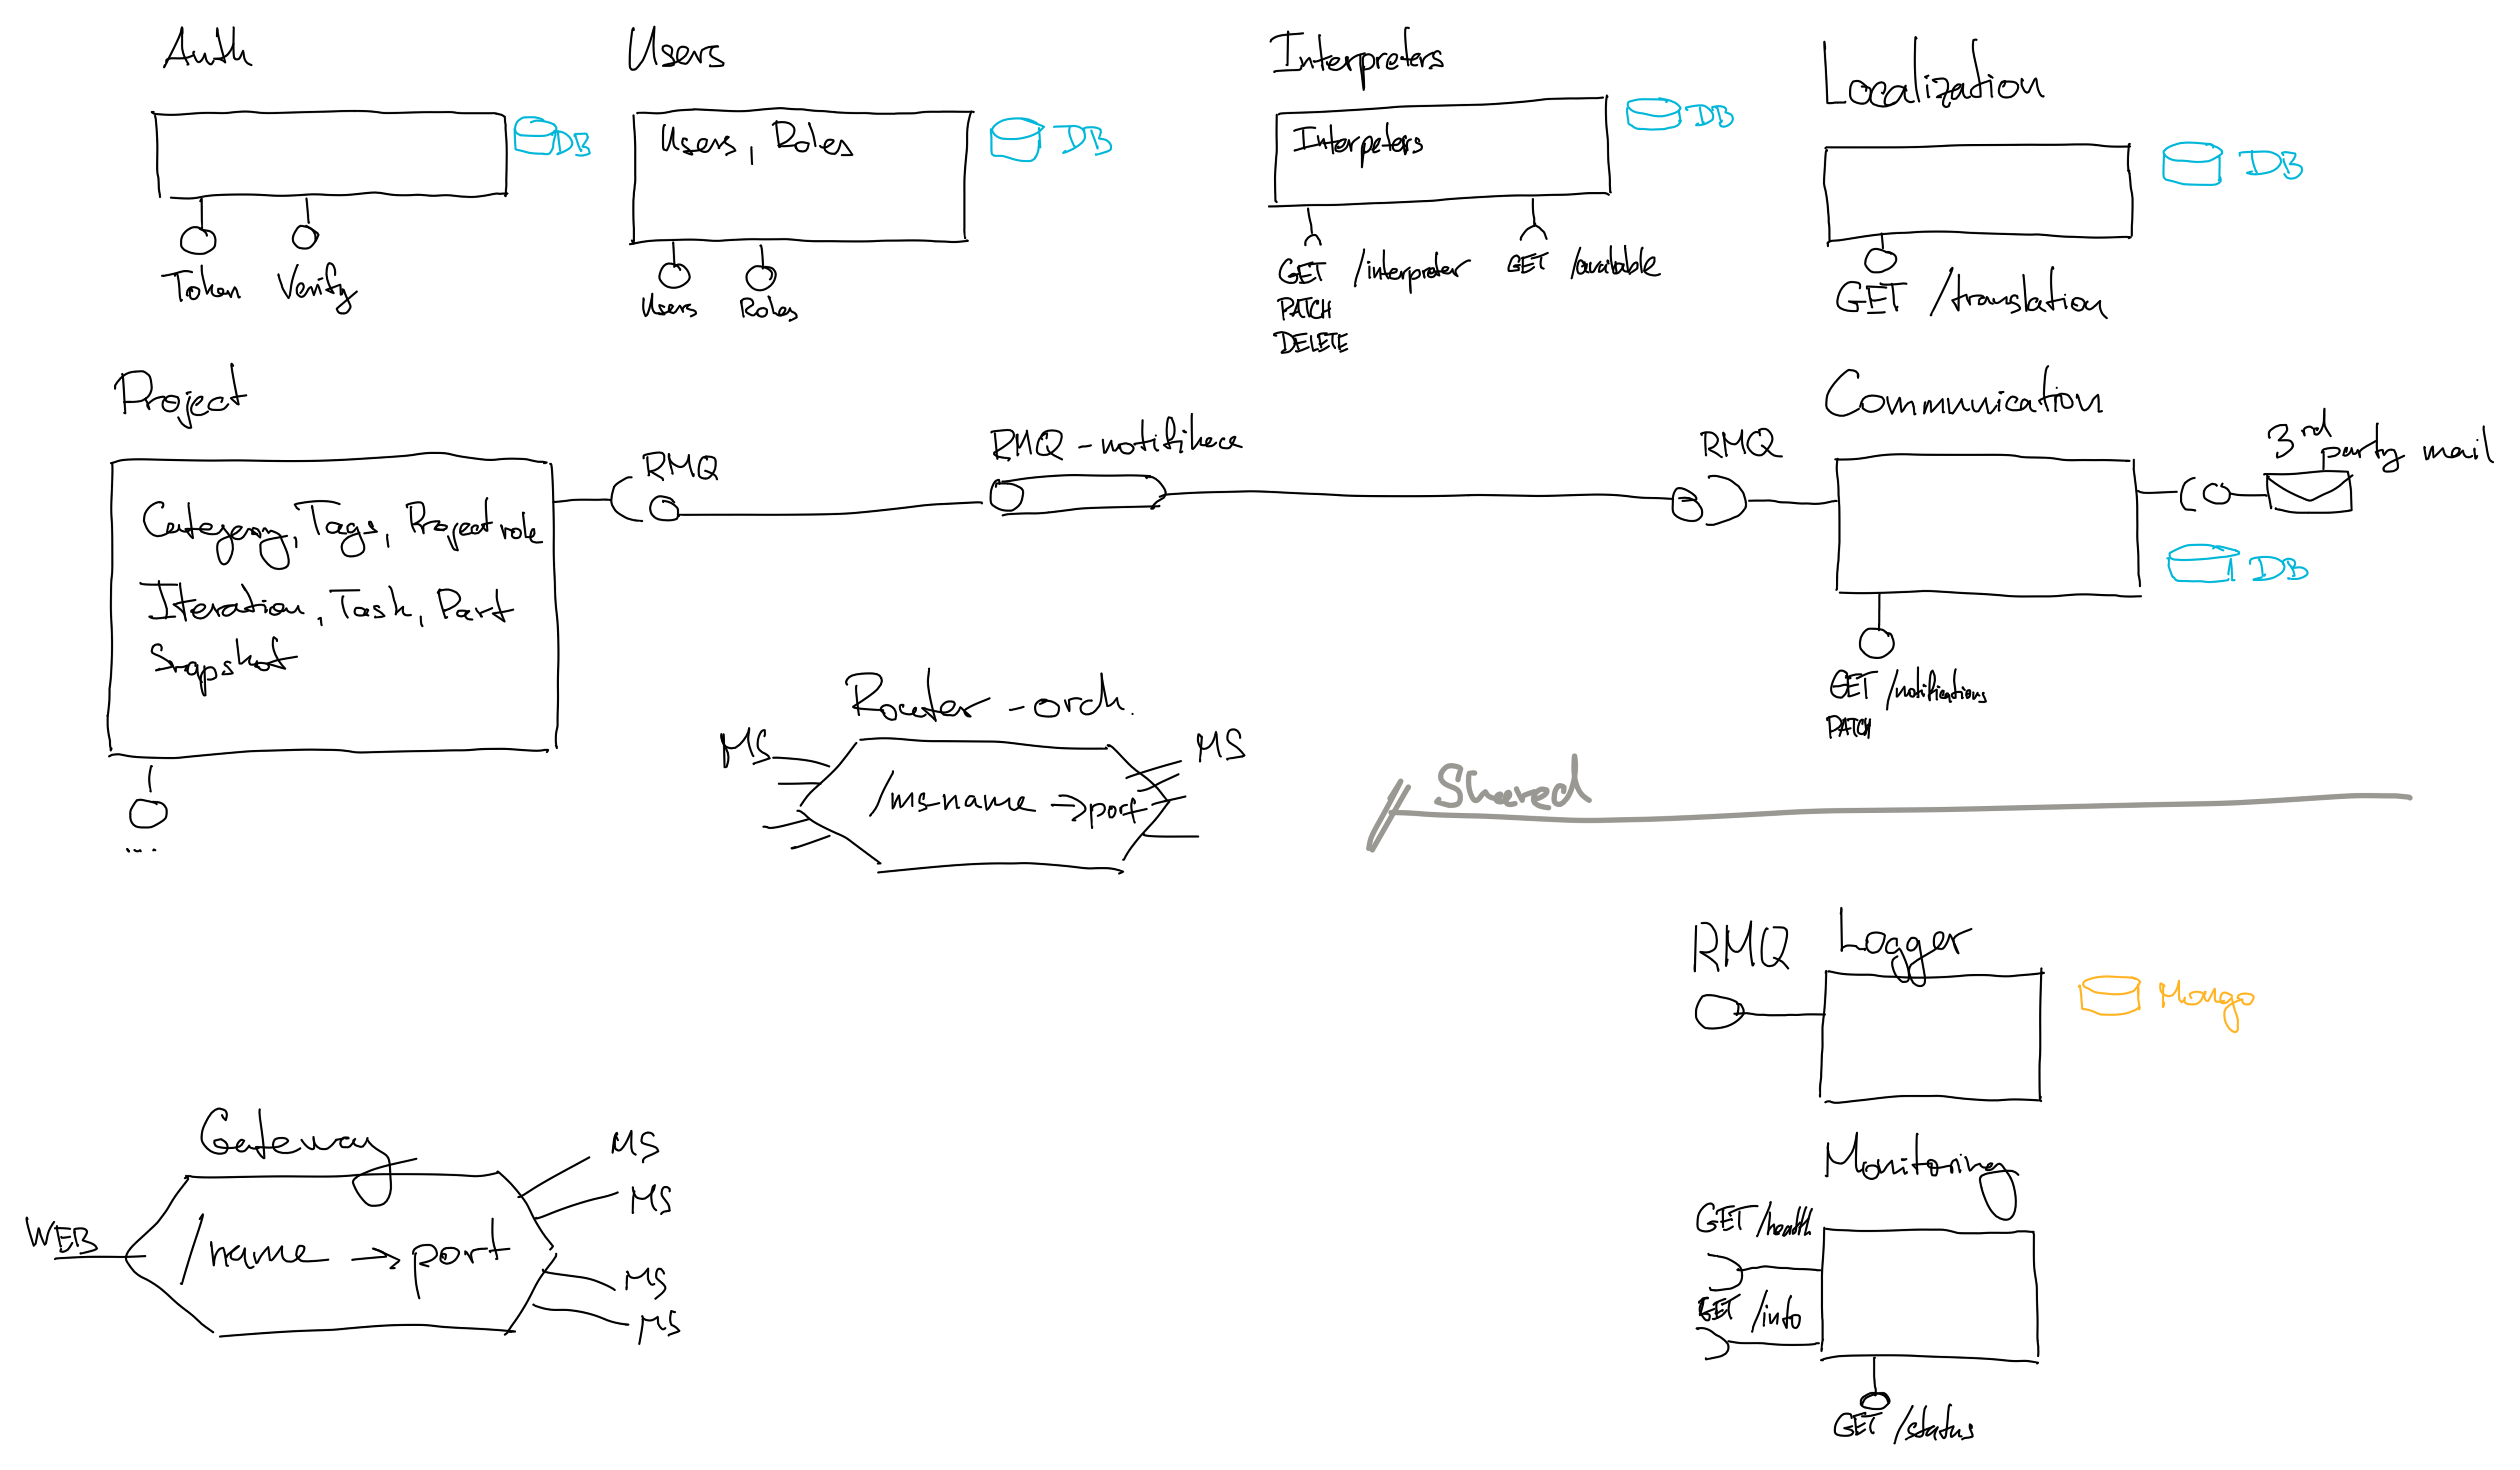
\includegraphics[max width=\textwidth]{assets/draft-server-arch}
   \caption{Architektura serveru}\label{fig:server-arch}
\end{figure}

\begin{figure}[htbp]
   \centering
   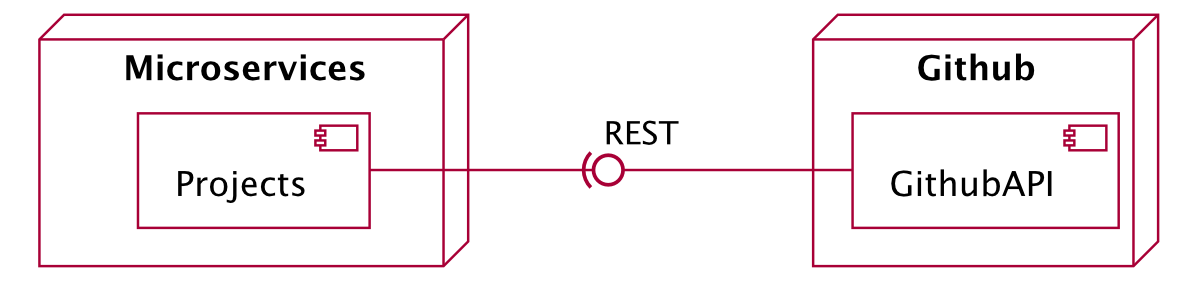
\includegraphics[max width=\textwidth]{assets/draft-be-github}
   \caption{Vazba mikroslužby na Github}\label{fig:server-github}
\end{figure}



\section{Šablona pro mikroslužbu}\label{sec:server-template}

Všechny mikroslužby v architektuře sdílí určité chování a poskytované rozhraní.
Vzhledem k požadavkům systému na základě předchozí analýzy byly vybrány následující návrhové vzory pro implementaci:
\TODO{seznam implementovanych vzorů}
Na obrázku~\ref{fig:ms-template} lze vidět vizuální znázornění rozhraní, které vzniklo jako následek výběru návrhových vzorů.


\begin{figure}[htbp]
   \centering
   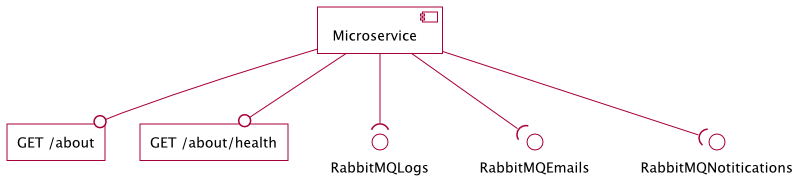
\includegraphics[max width=\textwidth]{assets/draft-ms-template}
   \caption{Standardizované rozhraní mikroslužeb}\label{fig:ms-template}
\end{figure}

Zarhnuje v sobě:

\begin{ul}
   \item \h{GET \g{REST} /info} pro získání základních metainformací o službě (například název, verze, vyžadované závislosti apod.),
   \item \h{GET \g{REST} /health} pro kontrolu, zda tato služba je dostupná,
   \item \h{RabbitMQ log} pro připojení se k RabbitMQ kvůli zápisu logů,
   \item \h{text log} pro běžnou kontrolu logů napřímo v \g{MS},
   \item jiné komunikační kanály pro poskytování svých možností.
\end{ul}



\section{Databáze a správa dat}\label{sec:server-db}

Pro správu dat v databázích byl vybrán vzor používající jednu databázi se sdíleným přístupem pro všechny \g{MS}.
Migrace


